\documentclass{article}
\usepackage{graphicx}
\title{Pinhole Cam}


\begin{document}
\maketitle
From wiki

\itemize
\item A 3D orthogonal coordinate system with its origin at O. This is also where the camera aperture is located. The three axes of the coordinate system are referred to as X1, X2, X3. Axis X3 is pointing in the viewing direction of the camera and is referred to as the optical axis, principal axis, or principal ray. The 3D plane which intersects with axes X1 and X2 is the front side of the camera, or principal plane.
\item An image plane where the 3D world is projected through the aperture of the camera. The image plane is parallel to axes X1 and X2 and is located at distance  f  from the origin O in the negative direction of the X3 axis. A practical implementation of a pinhole camera implies that the image plane is located such that it intersects the X3 axis at coordinate -f where f > 0. f is also referred to as the focal length[citation needed] of the pinhole camera.
\item A point R at the intersection of the optical axis and the image plane. This point is referred to as the principal point or image center.
\item A point P somewhere in the world at coordinate  $(x_1, x_2, x_3)$  relative to the axes X1,X2,X3.
\item The projection line of point P into the camera. This is the green line which passes through point P and the point O.
\item The projection of point P onto the image plane, denoted Q. This point is given by the intersection of the projection line (green) and the image plane. In any practical situation we can assume that $x_3 > 0$ which means that the intersection point is well defined.
\item There is also a 2D coordinate system in the image plane, with origin at R and with axes Y1 and Y2 which are parallel to X1 and X2, respectively. The coordinates of point Q relative to this coordinate system is  $(y_1, y_2)$ .
\begin{figure}[ht]
    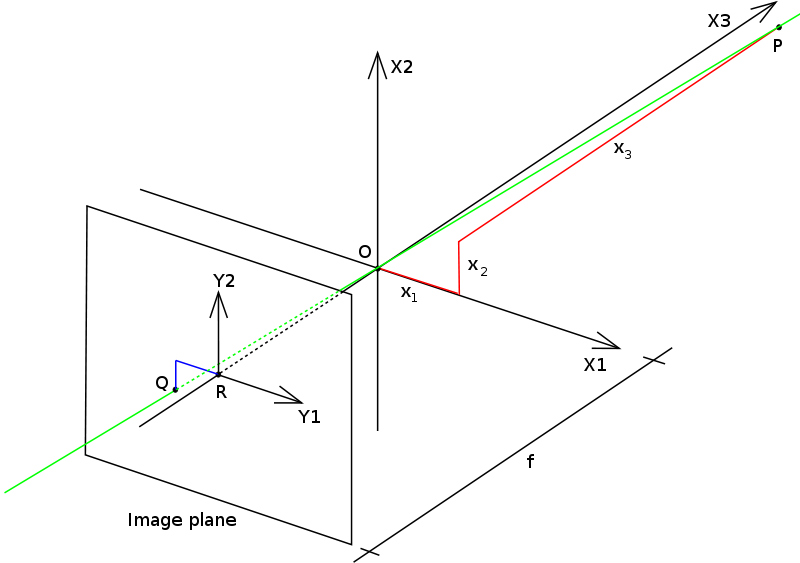
\includegraphics[width=.6\textwidth, height=50mm]{pinholecam.png}
\end{figure}
\end{document}


